% vim: set tw=78 sts=2 sw=2 ts=8 aw et ai:

The current implementation, although fully functional for the desired task,
has some inefficient resource usage and has been know to have periods when
performed below expectations.

In order to determine how to enhance VMchecker's performance, real life
statistics about how current VMchecker implementation performs. Taking data
from UPB Computer Science Department courses during an academic year and
analysing the number of submissions, the submission time, the duration of
the evaluation, we can determine the possible bottlenecks of the system and
find the places where improvements can be made.

Logs from submissions from several courses have been taken under
consideration. These courses vary from basic programming, operating systems programming or
administration, network administration to algorithms. Each has certain
constraints for containment test time and storage. Some run simple tests
that take a short time, others run simple tests but take more time, some
run tests that need root access on the machine, some need an input of a
single source file, others need the input of an entire virtual machine of
several gigabytes.

All submissions are treated almost the same (the virtual machine possibly
being different) with a First Come, First Served policy. If the tester can
run a single test at any one time, because a single virtual machine can be
started on the tester, bottlenecks are formed.

The pattern of the submissions isn't a constant line. There are moments
(ranging from minutes to days) where the checker isn't used and others
where several submissions are made almost at the same time.

Using data from two courses that take place in the same semester, each with
10 homework assignments, the patterns can be simply analysed. During the
course of a semester (14 weeks) about 13300 were made, out of which about
12400 were valid and actually tested. The times of the submissions and the
duration until results came in for that submissions where taking into
account measure the load of the infrastructure.

Figure \ref{fig:sub} shows the evolution of the number of submissions over
the semester. It is clearly visible the fact that the number of submissions
increases as headline for assignments come near. If two deadlines for
different courses overlap within a couple of days, the number peaks.

The relationship between the number of submissions and the average time to
get the results is shown by figure \ref{fig:sub}. Because of the first come
first serve algorithm and the fact that there is only one tester for all
the submissions means that if the number of submissions increases
considerably. If the first homework in the queue takes a certain time, the
next one will take twice as long before the results for it are returned.

\begin{figure}[H]
\begin{center}
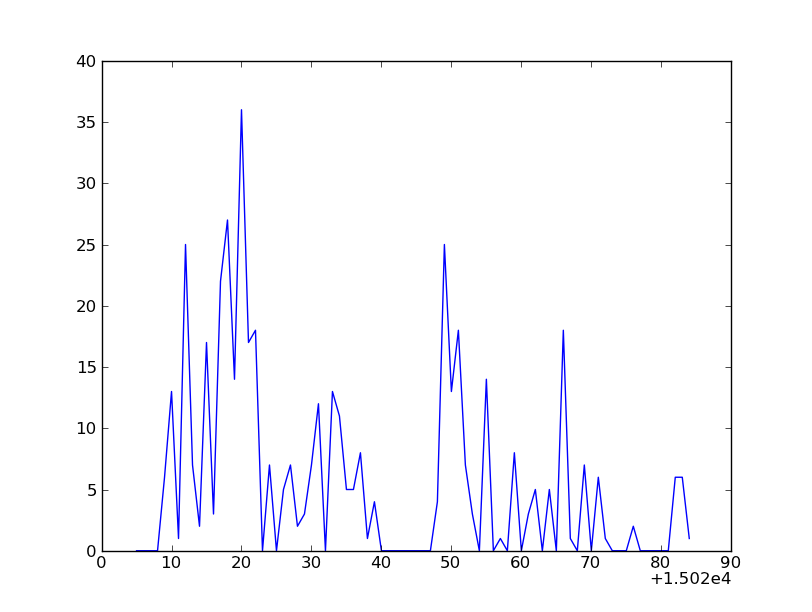
\includegraphics[height=0.4\textheight]{src/so}
\caption{Average number of submissions}
\label{fig:sub}
\end{center}
\end{figure}

\begin{figure}[H]
\begin{center}
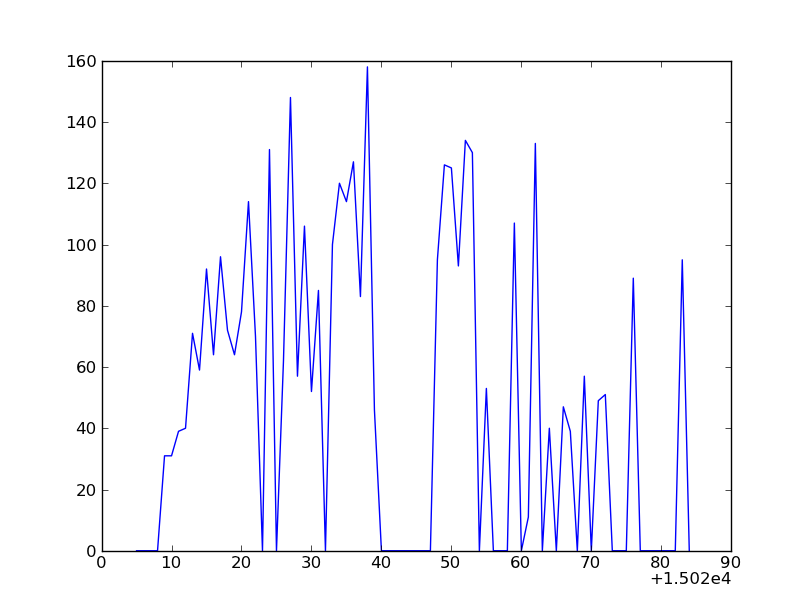
\includegraphics[height=0.4\textheight]{src/sotime}
\caption{Average time for testing}
\label{fig:time}
\end{center}
\end{figure}

